% EPL master thesis covers template
\documentclass{eplmastersthesis}
\usepackage{float}
\usepackage{xcolor}

% Please fill in the following boxes
% Title of the thesis
\title{Integrated mini-cloud of RaspberryPIs for distributed systems training}

% Subtitle - remove this line if not applicable
\subtitle{The Splay Project}

% Name of the student author(s)
\author{Rémy \textsc{Voet}}
\secondauthor{Samuel \textsc{Monroe}}		% remove if not applicable
%\thirdauthor{Firstname \textsc{Lastname}}			% remove if not applicable

% Official title of the master degree (copy/paste from list below)
% Master [120] in Biomedical Engineering
% Master [120] in Chemical and Materials Engineering
% Master [120] in Civil Engineering
% Master [120] in Computer Science
% Master [120] in Computer Science and Engineering
% Master [120] in Cybersecurity
% Master [120] in Data Sciences Engineering
% Master [120] in Data Science: Information technology
% Master [120] in Electrical Engineering
% Master [120] in Electro-mechanical Engineering
% Master [120] in Mathematical Engineering
% Master [120] in Mechanical Engineering
% Master [120] in Physical Engineering
% Master [60] in Computer Science
% Specialised master in nanotechnologies
% Specialised master in nuclear engineering
\degreetitle{Master [120] in Computer Science}

% Name of the supervisor(s)
\supervisor{Étienne \textsc{Rivière}}
%\secondsupervisor{Firstname \textsc{Lastname}}		% remove if not applicable
%\thirdsupervisor{Firstname \textsc{Lastname}}		% remove if not applicable

% Name of the reader(s)
\readerone{Firstname \textsc{Lastname}}
\readertwo{Firstname \textsc{Lastname}}			% remove if not applicable
\readerthree{Firstname \textsc{Lastname}}			% remove if not applicable
%\readerfour{Firstname \textsc{Lastname}}			% remove if not applicable
%\readerfive{Firstname \textsc{Lastname}}			% remove if not applicable

% Academic year (update if necessary)
\years{2018--2019}

% Document
\begin{document}
  % Front cover page
  \maketitle

  \chapter*{Abstract}

  \chapter*{Acknowledgements}

  \tableofcontents

  \chapter{Introduction}

    \section{Context and Motivations}

      {\color{red} Rewrite and complete this, placeholder right now}\\

      The process of learning distributed systems and algorithms is usually
      undermined by the difficulty of being able for one to test and apply
      what he learns.\\
      Indeed, in order to run a distributed algorithm and observe the result, a
      collection of machines running the algorithm is needed. Besides that,
      one would like to be able to change the conditions in which the algorithm
      is run, for example by provoking faulty nodes, or inducing network
      perturbations among the system, as distributed algorithms are designed to
      adapt to these conditions. These needs make it really cumbersome
      for students to setup a testing environment emulating realistic
      conditions for learning purposes.

    \section{About the Splay Project}

      % Discussion about what was available when we started the rework of the Splay project.
      The SPLAY project has initiated to solve the difficulty to test and
      develop distributed algorithm in a large scale. SPLAY is not a recent
      project (begin around 2006), and lot of features have been added during
      some years. The first version of SPLAY  was designed to "covers all
      aspects of the development and evaluation chain" of distributed
      application \cite{SPLAY}. \\

      After some years, a module has been constructed be to manage network
      topology, SplayNet \cite{SplayNet}. This middleware implements a easy
      way to set the topology network between the endpoints (machines) and
      restrict the usage of the network depending of that.

      \subsection{Legacy Splay Project}

        When we begin our work on Splay, the repository of the
        project \cite{SplayGit} was not consistent. Indeed,
        the master branch is unstable, ...

      \subsection{A first update}

        Nous avons eu la chance d'obtenir auprès de l'UCL un travail étudiant
        en lien direct avec ce mémoire. Il s'agissait, à l'issue de dix jours
        de travail, de mettre à jour la version des technologies utilisées par
        Splay et par la même occasion acquérir une connaissance plus complète
        du fonctionnement du projet.\\

        Lors du début du travail, les derniers updates sur le projet dataient
        de 2016, et un certain nombres de features et améliorations avaient
        été développés jusque là. Cependant le projet n'était pas dans un
        état stable et donc Raziel Carvajal Gomez (notre superviseur pour ce
        travail contributeur de Splay) a préféré nous faire faire un fork
        du projet sur un commit remontant en Septembre 2011.\\
        Nous avions donc le bénéfice de repartir sur des bases saines et
        un projet fonctionnel, mais avec une grande perte en ce qui concerne
        le travail qui avait été accompli sur les cinq années qui séparent
        2011 de 2016.\\
        C'est là que nous avons relevé le premier problème
        et élément que nous voulions absolument changer et intégrer dans notre
        reprise de Splay: le projet avait été transferé depuis son ancien
        système de versionning sur Git et uploadé sur Github en Juin 2011 mais
        n'avait pas profité du système de tag de versions offert par Git pour
        référencer dans l'histoire du projet des releases fonctionnelles
        et stables, c'est donc quelque chose que nous mettrions en oeuvre
        par la suite.\\

        Partant de là, nous avons pu nous familiariser progressivement avec
        le fonctionnement du projet et son architecture software, appréhender
        les différents services qui le composaient et comprendre leurs
        interactions. Une fois cette connaissance acquise, nous avons pu
        commencer à upgrader les différentes versions des technologies
        utilisées en commencant par le Ruby et le Lua, les deux plus importantes
        et plus présentes technologies du projet.\\
        Avec des versions datant de 2011 maximum, et étant donné que nous voulions
        transiter sur les versions les plus récentes disponibles, nous savions
        pertinamment qu'au moment où nous changerions les versions, le projet
        deviendrait totalement instables et que de nombreux appels de méthodes
        ou fonctions dépréciées seraient à changer avant de récupérer un état
        stable. Mais là aussi nous avons relevé un second problème et élément
        primordial à intégrer pour les futures améliorations, le projet
        manquait cruellement de tests, à quelque niveau que ce soit.\\

        La conséquence de ceci était que nous devions réparer pas à pas le
        projet suite au changement des versions des langages et frameworks en
        devant nous baser sur notre compréhension globale du projet acquise
        précédemment et sur des resultats finaux attendus lors de l'exécution
        de divers scénarios utilisant le projet. Il nous était impossible d'être
        certains que nos changements n'affectaient pas le fonctionnement interne
        du projet de manière négative mais imperceptible, conséquences qui
        étaient en fait inévitables mais que nous ne découvririons que par
        la suite lors de l'implémentation de nouvelles features.\\
        Il était dès lors évident pour nous que nous mettrions en place des
        séries de tests à plusieurs niveaux lors des prochaines phases du
        projet, afin de rendre celui-ci bien plus maintenable que dans l'état
        où nous l'avons repris et de pouvoir garantir de futures améliorations
        plus aisées.\\

        Nous sommes donc parvenus à progressivement remettre en état (partiellement avec la feature principal) de
        fonctionnement tous les éléments composant Splay avec les nouvelles
        versions, en mettant également à jour les librairies utilisées par
        les différents langages. Les changements principaux en termes de
        version de technologies sont les suivants :

        \begin{itemize}
          \item \textbf{Ruby}: 1.8.6 $\rightarrow$ 2.5.3
          \item \textbf{Lua}: 5.1 $\rightarrow$ 5.3
          \item \textbf{Rails}: 2.1.0 $\rightarrow$ 5.2.0
          % Eux, ça s'était après :
          % \item \textbf{MySQL}: 5.5 $\rightarrow$ 5.7
        \end{itemize}

        Nous avions à l'issue de ces dix jours de travail une base saine et
        mise à jour prête à être utilisée pour le travail concret de notre
        mémoire.\\

        En plus de ceci, une autre partie du travail a consisté, une fois les
        updates réalisés, à mettre à jour la documentation du projet et y
        décrire le fonctionnement des différents services ainsi que de prendre
        du temps afin de réfléchir à des améliorations au niveau de
        l'architecture du système et de son fonctionnement et avons émis
        les réflexions suivantes :

        \begin{itemize}
          \item L'organisation du code n'était vraiment pas idéale et devrait
          être changée. Le code des six différents services se trouvait dans
          un seul même repository, ce qui rendait compliqués la navigation dans
          l'arborescence du projet pendant le développement, le suivi des
          commits et donc de l'évolution de ces différents services.
          \item Le fait d'utiliser une database comme point de communication
          entre le côté user et le \textbf{Controller} n'était peut-être
          pas aujourd'hui la meilleure manière de procéder.
          \item L'utilisation de Ruby comme langage pour le \textbf{Controller}
          et de LUA pour les \textbf{Daemons} n'était peut-être plus
          aujourd'hui un choix pertinant et des alternatives possibles
          pour des applications multi-processus et concurrentielles telles
          que Elixir demandaient analyse. Un différent choix de technologie
          aurait aussi pu par la même occasion solutionner notre interrogation
          précédente sur la base de données.
        \end{itemize}

        Ces réflexions ont été ensuite discutée avec Etienne Rivière, afin de
        dresser ensuite le ligne directrice et les objectifs concrets à atteindre
        pour la suite du projet et entammer la version 2 de Splay.

  \chapter{Splay Version 2} %TODO: Review - Rewrite

    % All about what we wanted to do exactly.
    Then, our goal for the new version of Splay, was first, stabilize and
    modernize the legacy project. Indeed, some parts was not updated or
    partially documented. All details is available in the next section.\\

    In a second step, we wanted to add our own features focus on the usage of
    the final user (student, professor or searcher). These features were a
    modern web application with Lua editor integrated, a graphical topology
    creator inside the web app and a way to inject some fault injection in the
    user code. We will details all of then in this chapter.

    \section{Objectives} %TODO: Review - Rewrite

      % Adding features of splayNet with
      Our Objectives can be easily cup in two parts, first the maintainability
      of the project and the new features added (next section). The section
      about our first update during a student job, explains the upgrade of
      language version but this upgrade was not covered all features of the
      legacy project (example: SplayNet). Then our first job was to
      \textbf{complete the missing features} done after  September 2011.\\

      % Raspberry
      The first idea of our master thesis was able to run Splay on a
      \textbf{cluster of Raspberry Pi}. The configuration of this cluster won't
      be trivial : one Raspberry need to be the master and able to control the
      rest of the cluster. Then the master need to run the controller and the
      web application and the other need to be handle to manage several Splay
      daemon (use as a machine for the distributed algorithms). \\

      % Clean code source - repo
      Secondly, Splay is not a small project, and several technologies
      (services) orchestrated between then. For this reason, the source code
      architecture is very important for the project maintainability. In the
      legacy project all code was on a single git repository host on Github,
      but this one is a "mess". The documentation is not in the right place,
      the logic of the directory structure is too complex, ... Then we wanted
      to do a better \textbf{management of the source code} and documentation
      readable by someone finding our repository. \\

      % Easy installation : On click install : docker (independent of OS), installation script,
      During our first work on Splay, we noticed that the installation and the
      usage was not quite easy to handle. Some services were dockerize and a
      docker-compose file was implemented which facilitate the installation.
      But these docker images were not perfectly build : healthcheck missing,
      old base image in some cases or big distribution base image (slow and
      take place). Also there wasn't a proper \textbf{one-click install}
      script for making quick test. Then, one of our goal was to get clean,
      small and with updated libraries docker images. These images need to be
      fully integrated between then through the docker-compose. A automate
      install script and running script, will be appreciate and useful as a
      example for the user.\\

      % Bug track - Testing - Solve issues of the old project
      Our first issues encounter with Splay, was the lack of
      \textbf{automatic tests} in all part of the project and because of this,
      there were a lot of silent bugs scattered in all the project.
      Accordingly, we wanted to upgrade the robustness of the project,
      it is means create specific test for critical parts and the main features
      of Splay. Two type of test can be created, local testing and integration
      testing. The first type allows to test a specific critical part or
      feature of one service (independently of others). The second kind is
      testing the global project by simulate a real user and getting real
      result from Splay (able to test the chain of service). The goal of these
      test is a better bug track and create maintainable project for future
      development.\\

      % Merge Web app and Cli server + new web app
      During our student job, we observed some code repetition and service
      repetition (cli server and the old web application). Then,we wanted
      to \textbf{avoid the repetition of job} (and code by extension) by
      change these services or merge it. Again, the purpose was the
      maintainability and refactor some old code. Moreover, we wanted to
      modernize the web application of the legacy project and add some
      features on it (next section)


    \section{New features of Splay} %TODO: Review - Rewrite

     To present our own new features of Splay, we will explain by some user
     scenarios and after explain in details the three features.

      \subsection{Scenarios} %TODO: Review - Rewrite

        \textbf{First Scenario : } as a student, I want to put in practice my
        course on distributed application. The university provides a existing
        installation of Splay in the local network. The student just need to
        connect on the web server with its browser. The student, after
        registering, will able to create its own code with a complete Lua
        editor on the web page. Also a powerful and documented library
        facilitates the creation of distributed algorithm. When the code is
        finished, the student launch the job, the code will be automatically
        dispatch on several machines (depending of number of available daemon
        and the number choose by the student), and getting the log of each of
        then in the web page during/after the completion of the algorithm.
        Also, if it is too long the student can choose to kill the job. The
        student, through a simple web interface, can put in practice its course
        and see the result quickly via logs.\\

      	\textbf{Second scenario : } a professor wants to test a new approach to
        solve the problem of leader election between multiples nodes. A cluster
        of Raspberry is set up with Splay to make the experiment. The new
        approach is described in a paper with some pseudo-code and some difficult
        cases when the network topology is quite exotic. Then the professor need
        to rewrite the pseudo code in a actual one, and create a simulation for
        each different network topology to point the strength of this new
        approach. Unfortunately, He is very busy, and his/her time is very
        precious. It is the case where Splay can be the solution, it manages
        network topology transparently and give a topology creator in a web page.
        Also the library of Splay in the Lua side allow to quickly reproduce the
        pseudo-code.

        % \textbf{Third scenario : } A employee from a big cloud company want to test the robustness of their new Top Secret distributed algorithm. TODO

        % as a employee from a cloud company who want test the robusness of their new Top Secret algorithm.

      \subsection{Details of features}  %TODO: Review - Rewrite

        \subsubsection{Complete Lua editor on the website}  %TODO: Review - Rewrite

        Splay in version 1, had a web application, with some basics features :
        user connection, list of job, creation of job and a way to retrieve
        logs. This web application as explained before was very trivial with
        almost no CSS and poor in term of content. Then, we wanted to refactor
        completely and modernize the old web application. And, also in this
        purpose, the user could use a integrated Lua editor directly on the
        website. This editor should be standalone, with coloration for Lua
        language, error parsing and maybe some small auto-completion. This one
        need to be integrated into the form of the job creation.

        \subsubsection{Topology creator/visualisation} %TODO: Review - Rewrite

        Also, the legacy project manages network topology. Indeed a user can
        defined its own network topology with different settings for each
        edge : the latency, the bandwidth and error dropping packet. Also it
        is possible to make more complex network by adding router between nodes
        and Splay will approximate the true parameters for each
        source-destination (Splay will not simulate the internal node of the
        network, for performance reason and simplicity). \\

        The network settings is done on the legacy project by a XML file with a
        specific format (ModelNet \cite{ModelNet}). This format is not user
        friendly and hard to read, also the documentation is poor. For these
        reason, we decided to add a visualization and creation tool of the
        network graph. Then, it will be possible to create easily a visual
        topology with all type of setting and it will be transform
        automatically in the correct format of XML. But`, the opposite will be
        possible, it means from a XML, see the topology into a graph
        representation.

        \subsubsection{Fault Injection} %TODO: Review - Rewrite

        The creation of distributed algorithm is a difficult task, and
        moreover, it is hard to make real code who is reliable. Robustness
        and correctness of a distributed solution is the key point to test
        for a designed solution, and manually injection of fault is painful
        and can take some time. \\

        With the legacy project and the dockerization, it was possible to
        crash a single daemon during the execution of a job. But the main
        problem of this solution, we can't control where the crash is done
        (in the execution tree). We wanted to improve this precision by adding
        a feature where the user is able to choose when a daemon (or several)
        crash during the execution of code. It need to convert the two main
        different, the hard crash (the nodes is destroyed) or a recovery crash
        (nodes crash but it is relaunch after some time). \\

        To resume, the fault injection will allow (user) to choose when (in
        the execution tree) and where (one or several nodes) the crash is done
        in the daemon, specified the type of crash and act depending. This
        possibility for the user need to be user friendly and quick to make.

        % This for reason - 2 types of crash possible - can touch one or more than one in the same time - crash in middle 2 instruction.

  \chapter{Architecture}

    \section{Software Architecture}

      It is important here to discuss about the software architecture of the
      Splay Project as it has impacts on the way we achieved this work

      \subsection{Legacy Architecture}

        The old Splay architecture was composed of :

        \begin{itemize}
          \item The \textbf{Controller} : The core part of Splay, waits for jobs
          and dispatch them to the daemons.
          \item \textbf{Daemons} : Workers registering to the controller and waiting
          for jobs to achieve.
          \item A \textbf{MySQL DB} : The communication piece of Splay, allowing
          communication between the user and the system.
          \item A \textbf{CLI Server, CLI Client, SplayWeb} : Pair of CLI tools
          and a web application made in Rails to let user interact with
          Splay through communication with the MySQL Database.
        \end{itemize}

        \begin{figure}[H]
          \centering
          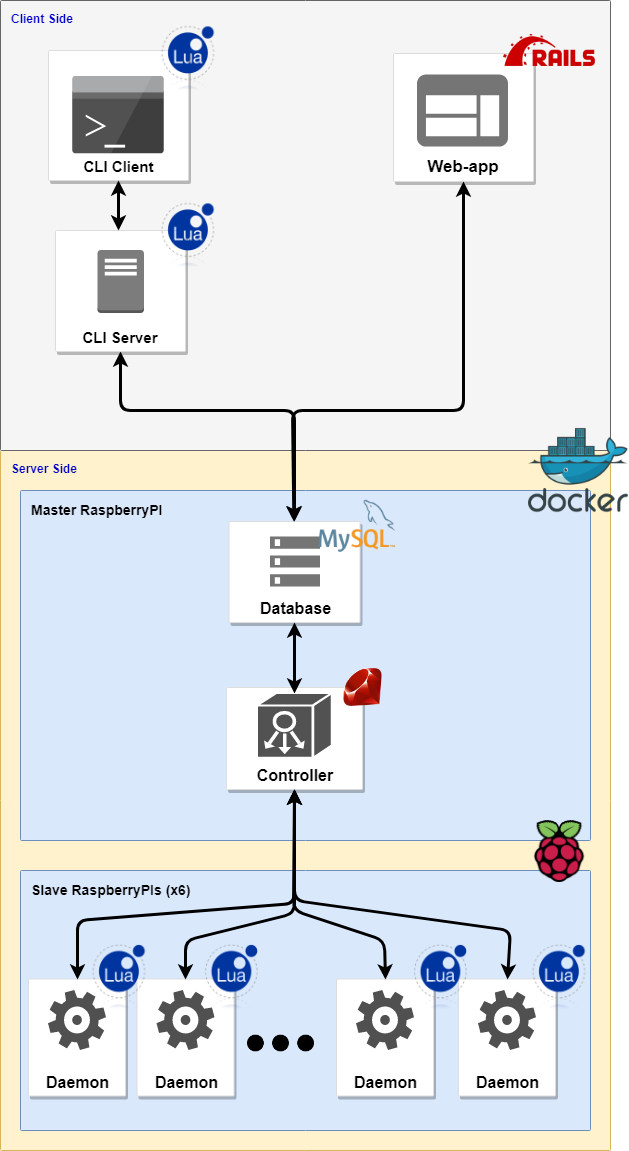
\includegraphics[scale=0.6]{figures/prev_arch.png}
          \caption{\label{prev_arch} Previous Splay Architecture}
        \end{figure}

        Whether through the usage of the CLI application or the web application,
        the user was able to interact with the Splay system and to send his
        jobs, and gather many informations such as the logs or the current
        state of the running Splayds (the Splay daemons).

        The fact that the database was the central piece of communication
        between the controller and the user applications was a design choice
        that we decided to respect and to keep working that way. Indeed, the
        \textbf{Controller} is the central piece within the Splay project,
        trying to push changes in that design choice and try to implement a
        different way of communication than the database would have, more
        than probably, implied a total rewrite of the controller.\\

        That being said, we weren't totally satisfied about the interaction
        possibilities offered to the user. Indeed, the Ruby on Rails application
        was quite old, and the client/server pair of the command line interface
        stack had a hard to maintain and to huge codebase compared to the
        features that it had to offer.\\

        We thus chose to operate major changes on this part of the Splay
        project, in order to combine the arrival of our new features and
        changes onto the core of Splay with a better user experience.

      \subsection{Renewed Architecture}

        The main issue on the architecture of the user services was a code
        duplication issue, or at least a duplication related to the solutions
        created to resolve a common problem. The Rails web application and the
        CLI server had the common role of letting the use manipulate the
        database to transmit and gather informations to the \textbf{Controller}.\\

        The first decision to make in order to solve this problem was to
        merge those two services into a single one and to call that new
        service according his role among the system: the \textbf{backend},
        according to the viewpoint of the client.\\
        This backend would have the ambition to offer a secured API through
        the usage of JWT \cite{JWT} and therefore allowing the development
        of services around that backend, in our case a web application and
        a command line interface application.\\

        The web application would thus use a recent JavaScript technology
        allowing dynamic interactions with the user, and the CLI would use
        a simple and dedicated technology, those two services consuming the
        same API offered by the backend. The backend, for its part, would
        stay in the Ruby ecosystem, in order to keep a technology concistency
        with the global project and the technologies already in use.\\

        The resulting reworked architecture would therefore be the following :

        \begin{itemize}
          \item The \textbf{Controller} : The core part of Splay, waits for jobs
          and dispatch them to the daemons.
          \item \textbf{Daemons} : Workers registering to the controller and waiting
          for jobs to achieve.
          \item A \textbf{MySQL DB} : The communication piece of Splay, allowing
          communication between the user and the system.
          \item \textbf{Backend} : The backend of the client side Splay app
          \item A \textbf{Web-app} : The single-page application
          \item A \textbf{CLI} : The command-line interface
        \end{itemize}

        \begin{figure}[H]
          \centering
          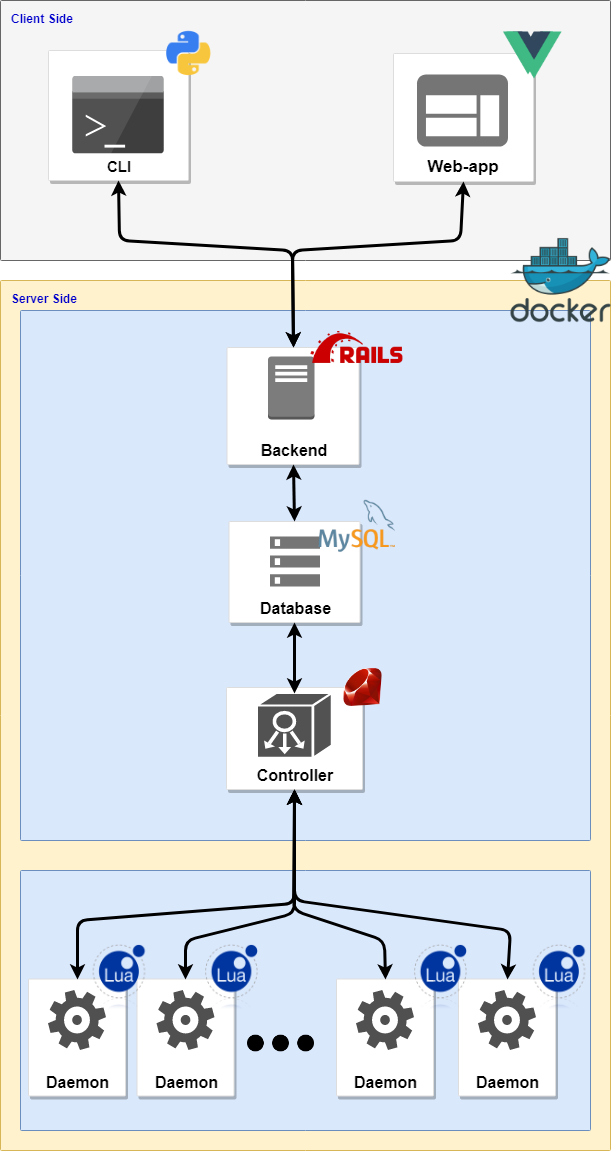
\includegraphics[scale=0.125]{figures/new_arch.png}
          \caption{\label{new_arch} New Splay Architecture}
        \end{figure}

    \section{Hardware Architecture}

      About the Rasp cluster.

  \chapter{Development Methodology}

    Before speaking about the implementation details, it may be useful to
    describe the way we organized ourselves in order to develop the application.
    The fact of being two student on this development project necessarily
    implied a way of organizing ourselves a bit more serious than a
    development project alone.\\

    Thanks to the courses about AGILE methodologies we followed during our
    scholarship, and the both of us having had the occasion of acquiring
    experience in a professional way through internships and part-time jobs,
    we wanted to put to work this knowledge and good practices acquired in
    the project management domain.\\

      \section{Kanban}

        The first tool we put in place, and this from the very beginning of
        the update period of Splay about which we talked in the previous
        sections, was a Kanban using the online website Trello \cite{trello}.
        The kanban allowed us to : \\

        Le premier outil que nous avons mis en place, et ce dès notre période
        d'update de Splay dont nous avons parlé plus tôt, a été un Kanban en
        utilisant le site en ligne Trello. Le kanban nous a permis de : \\

        \begin{itemize}
          \item Have a clear and precise view about the remaining tasks we had
          to achieve in the backlog, and also about the development state of
          all the other tasks.
          \item Encourage and even oblige ourselves to translate the features
          we had to implement into sufficiently detailed and explicit cards on
          the kanban. This process has the benefit of refining or making
          features the most explicit possible before starting the development.
          \item Have a way of tracking the project's progression and offering
          to all the people related to the project a simple and effective way
          to keep themselves informed about Splay's state.
          \item To focus ourselves on specific tasks and to work in an
          iterative and efficient way.
        \end{itemize}

      \section{Quality Assurance}

        Ceci sera explicité plus en détail dans un chapitre suivant, mais nous
        avons voulu nous assurer de maintenir un certain degré de qualité dans
        notre travail sur Splay et plus spécifiquement au niveau du code, afin
        aussi d'assurer la maintenabilité du projet. Nous nous sommes donc
        fixés ce but à travers la mise en place des éléments suivants : \\

        \begin{itemize}
          \item \textbf{Testing suites} : Ensembles de tests unitaires et
          d'intégration, intra-service et inter-services.
          \item \textbf{Linter} : Analyse statique du code afin de satisfaire à
          des exigeances de style de code et de bonnes pratiques.
          \item \textbf{Coverage Analyzers} : Analyse du pourcentage de couverture
          du code par les suites de tests.
        \end{itemize}

      \section{Github and Gitflow}

        The project and all the services composing it are versioned using the
        \textit{Git} versioning system and are hosted on the online service
        \textit{Github}.\\
        We therefore organized our work on the Gitflow model. Each feature or
        tasks we created on the kanban was meant to receive its very own
        branch, starting from the main branch.
        Once the feature finished and tested, a pull request was made asking
        to merge the feature branch with the main branch.
        The first benefit of this was obviously to keep the main branch in
        a working state with healthy and finished features.\\

        The second benefit of this way of working on the project was to
        permit, once again towards the goal of ensuring quality, code reviewing.
        Each time one of us was done with the development of a task and was
        issuing a pull request, the other was assigned as code reviewer and
        was in charge of making this code review, accepting the pull request and
        doing the merge, or to detect errors or bugs as the outcome of the
        code review and therefore to ask for changes to the pull request issuer. \\
        Besides the main code review's benefit of reducing the number of errors
        or bugs, this process also allowed each of us to keep itself aware and
        keep itself up to date with all the different changes happening on the
        different services. Indeed, it was impossible for us to work together
        in the mean time on each single service, because of the number of
        services and inter-dependant features we had to develop.

  \chapter{Implementation}

    \begin{itemize}
      \item Implementation choices details
      \item Story-telling about the development phase itself
      \item Details about the implementation, about how Splay is working today.
    \end{itemize}

    \section{Technology choices}

      \subsection{VueJS - Web App}

        As we made the decision that the web application would only be a
        front-end application making use of a centralized backend offering
        a complete JSON API, we canted to use a front-end web development
        framework that would satisfy the following conditions : \\

        \begin{itemize}
          \item Light
          \item Ease of development and maintenance
          \item Access to numerous third-party libraries
          \item Popular enough to be ensure support over time
        \end{itemize}

        In order to develop a front-end application, the JavaScript ecosystem
        was an obvious choice, and we made a pre-selection among the most
        popular web framework on the market and recognized for their qualities:
        ReactJS, Angular and VueJS.\\
        We rapidly removed Angular from our list because we preferred the
        component-based UI development offered by the two other frameworks,
        which were lighter and avoiding to have to develop in the MVC style.
        Even if we both had a previous experience with React thanks to a
        Cloud Computing course at the UCLouvain, we decided to go for VueJS
        instead of React.\\

        The first major advantage of Vue is how light it is, we also took into
        account the fact that this technology was gaining in popularity for
        multiple years now to be today a huge player in the world of the web
        technologies. Moreover, as we took some time to develop a proof
        of concept application using Vue, we were totally satisfied with the
        simplicity of development that that framework was offering to the
        developers and allowed us to be totally confident into the fact
        that going for this technology would allow any further contributer
        of the Splay project to easily get in and participate to the
        development.\\
        Indeed, a Vue application is organized around single components, each
        having their own HTML template, their CSS style declarations and
        the associated JavaScript code. No other exotic language is required.\\
        The fac tthat the framework is in the JavaScript ecosystem and
        associated to the NPM package manager also allow to take advantage of
        numerous existing libraries, such as data visualisation libraries,
        testing libraries, etc... \\

        For all those reasons, Vue revealed itself the best choice for a
        web application, and also allowing us to develop with a something
        we liked and with recent technologies, besides providing an efficient
        solution to the conditions we needed for the technology.

      \subsection{Python - CLI}

        The old pair of services intented to compose the CLI service was
        written in LUA on the client side, and the CLI server was in Ruby. As
        the server's logic would be moved and merged into the \textbf{Backend}
        service, and as we wanted to keep a command line interfact application
        in order to run tests of the global project, we needed to reevaluate
        the relevance of the LUA usage for this application.\\

        It is more than probable that LUA was used for coherence reasons back
        in the days, and to avoid to scatter Splay around too much different
        technologies (although Ruby may have been used too instead of LUA).
        Still, maybe today this choice was not the most relevant for a CLI
        application. Indeed, our small client CLI had to be :

        \begin{itemize}
          \item Simple
          \item Concise
          \item Written in an easy-to-use language
          \item Having conveniant libraries allowing to create simple CLI apps
        \end{itemize}

        However, we inherited of an application scattered in multiples LUA
        files, each file representing a CLI command. We therefore had a huge
        source of code duplication, as each file was repeating the process
        of parsing the user arguments when the program was called, and also
        repeating the process of reaching the server through a HTTP library
        in LUA.\\
        Ruby was indeed a relevant option if we wanted to restrict the number
        of different technologies in use among the project, but Python was
        a better choice to write such a simple script as our CLI. Python has
        a lot of very conveniant libraries to treat HTTP calls and to
        manage and parse user arguments when creating a CLI application.

      \subsection{Ruby on Rails - Backend}

        The controller service and the old pair of services composing the CLI
        having been developed with the Ruby language, and the old web
        application having been developed with Ruby on Rails, it was obvious
        for us to stay within the Ruby ecosystem to create the new service
        that would become what we called the \textbf{Backend}. The technology
        we wanted to use for this development had to offer an efficient
        solution to the following issues :

        \begin{itemize}
          \item Allowing a simple interfacing with the MySQL database in order
          to ensure the communication with the controller, and therefore allow
          the submission of new jobs, the gathering of information about the
          Daemons, etc...
          \item Allow to develop and expose a JSON API alloing other front
          end services (web application and CLI) to make use of this API and
          interact with the Splay system.
          \item Offer a large choice of libraries for testing, data
          serialization using JSON, and other libraries solving the problems
          we talked about before.
        \end{itemize}

        The both of us already having a certain experience in using Ruby on
        Rails, and for the reasons of ecosystem consistency we talked about
        in the previous sections, we immediately agreed on using this
        framework for the backend. The fact of staying in the same language
        ecosystem would allow us to make sure that future contributers to
        the application would not have to play with too many technologies and
        therefore make the future evolution of Splay easier.\\
        It should also be noticed that, as we exposed it when talking about the
        changes in the renewed software architecture of Splay, the previous
        web application and the CLI server had a similar role although being
        specialized for different applications. However, the commom logic
        of these two Ruby services was already present, and a part of the
        work was therefore just the matter of isolating this common logic
        and making it better.\\

        Indeed Rails allow to easily develop, besides traditional MVC web
        applications, API only applications that doesn't contain all the stuff
        and complexity needed for presenting HTML views to the user and thus
        having a lighter and more concise codebases.\\
        The ActiveRecord \cite{activerecord} ORM shipped with the Rails
        applications is also a major advantage for this technology, allowing us
        to easily and efficiently manage the system's jobs and daemons.\\
        Finally, the availability of some libraries such as RSpec made for the
        testing (topic on which we'll talk more deeply in a dedicated chapter),
        Rubocop for the linter, or even the Netflix's fast\_jsonapi library for
        data serialization has definitely made Rails the right technology to
        choose for the Backend.

    \section{Development}

      This section details in a story-telling way all the different part
      of our work on the project, starting from the first big code cleaning
      and refactors and ending with our latest features on the application.\\

      The organization of the section doesn't reflect a strict timeline of
      our work but is organized by date of beginning. Indeed, some goals
      and features needed further improvement over time.

      \subsection{Github Repository Reorganization}

        From our first analysis during our part-time job period on the Splay
        project, we weren't satisfied about how it was maintained on Github so
        far. Our major concern were the following :

        \begin{itemize}
          \item Lack of version tagging to specify stable versions
          \item The code organisation was not good and it was hard to
          understand exactly where the different services were located,
          everything was more or less in the same source folder.
        \end{itemize}

        From our last experience we also realized that the project was really
        lacking of documentation in order to help and guide people interested
        in Splay to install and run it.\\

        We therefore started with forking the project in a personal repository,
        allowing us to perform complete reorganization of all the directories
        and files composing the project and adding some basic documentation.
        Each service was successfuly placed in a distinct directory while
        keeping the docker-compose file working.\\
        The project was cleaner, however, we felt that this wasn't enough
        and that we could achieve a better structure. The project is big and
        consisting of multiple services interacting with each other but
        not sharing any code. We therefore decided to create a new Github
        organization called \textbf{The Splay Project V2} in which we created
        a distinct repository for each service and one as the main repository
        of the project.\\

        The main repository called \textbf{Splay} contains all the other services
        through the submodule \cite{GitSubmodules} feature of git. These
        subrepositories representing the new architecture wanted :

        \begin{itemize}
          \item the cli (command line interface)
          \item the daemon (also called \textit{splayd} in the project)
          \item the backend (the merge of the cli\_server and the old web app backend)
          \item The controller
          \item The new web application
        \end{itemize}

        Each of these subrepositories is self-sufficient and contains a Dockerfile
        allowing the user to create the related container and to use and test
        the service alone, and therefore also has it's own documentation.\\

        For each master branch of these subrepositories, a link with Dockerhub
        has been made so that each push on master will trigger an automatic build
        of a docker image using the source and uploading it on the Dockerhub \cite{DockerHubGithub}.
        This was especially made to ease the integration testing using a
        continuous integration service, which would have to build every single
        image otherwise.\\

        Now the services were clearly and logically separated in their
        distinct repositories, it would be really easier for us to track
        the changes made in each service and would ease further improvement
        by Splay maintainers.

      \subsection{Centralization of Splay's Backend}

        As said before in the technology choices section, one big thing
        we wanted to achieve was the merge of the old CLI server and
        the backend part from the full-stack old web application as those two
        services were basically achieving the same work and holding the
        same responsibilities.\\

        We started with a fresh Ruby on Rails application, passing the
        generator the \textit{--api} option so that we were provided with
        a clean and simple Rails app without all the front-end dedicated
        files, making it simpler and lighter.\\

        Before writing any line of code, the following tools were added
        to the project :

        \begin{itemize}
          \item \textbf{Rspec}: A performant and easy to use Ruby testing
          framework to be able to begin development following the test
          driven development approach.
          \item \textbf{Rubocop}: A static code analyzer (linter) to follow
          good codestyle conventions and avoid bad pattern right from the start.
          \item \textbf{Travis}
          \item \textbf{CodeCov} A test coverage tool to get further
          information on the test suite.
        \end{itemize}

        Now that the app was ready for development, the major features
        we wanted to provide were the one provided by the old CLI server and
        were the following :

        \begin{itemize}
          \item User and session management (creation, login)
          \item Job management (creation, deletion, listing, details)
          \item Daemon querrying (listing, details)
          \item Job logs querrying
        \end{itemize}

        Implementing those features would let us immediately reuse the old
        CLI client for testing purposes and would provide sufficient actions
        to start the development of the web application, which could unveil
        need for new endpoints on the backend to provide user with more
        actions in order to interact the system.\\


      \subsection{A new front-end application} %TODO: Review - Rewrite

        % maybe screen shots ??

        As the backend was available (previous section), we begon the
        developement of the Single Page Application in VueJS. After removing
        old files of the previous web site, we created a basic VueJS project
        (version 2.5.X at this time) with the home page and the bootstrap-vue
        package \cite{BootstrapVue}. \textbf{Bootstrap} \cite{Bootstrap} is a
        well know HTML, CSS, and JavaScript framework to create responsive and
        modern web interface. The full integration of bootstrap in a Vue
        project is done with the extension of bootstrap package, bootstrap-vue.
        For us, Bootstrap is like a Swiss knife to make a web page with minimun
        design and modernity. \\

        The next step was to build a register and login page for the user
        management. To manage different page in the same Vue project, we
        installed the Vue-Router package. It is a extension of Vue to navigate
        through different pages (url) on the single page app (no reload with
        the server), and the user can switch page as he was on a regular
        website (backward/forward page, historic, ...). It is commonly used in
        front end framework to give a better user experience. Then, we created
        a page for the user registering and connection, directly connected to
        the backend user API. For the json communication with the backend, we
        used axios \cite{axios}, a popular HTTP Javascript client. At the end
        of this version of the web application, the user can create his/her
        account and connect to it, and the token of authentification (token
        based authentification) will be save on the client browser (auto-login
        for the next visit). \\

        % job - splayd list and job form
        In order to get the same features as the legacy website, we created a
        monitor page, where important information is given with lists. Indeed,
        a list of splay daemon (create by controller) is retrieve from the
        backend and print with global information in a nice bootstrap table.
        Also, a second table, used for jobs (also via the backend service), is
        builded with general data. The user can choose to see more details on
        one splay daemon or a job via a button. Also, he can choose to kill a
        job through a red button, the controller will do the rest. Moreover, The creation of job is done
        with a simple form and it is automatically checked with vee-validate
        package \cite{VeeValidate} (also checked in the backend service of
        course). Vee-validate is a small package solutionning the problem of
        manual checking of form by adding some propreties to inputs, and it
        makes our code more compact and less messy. At this step, we had
        almost all legacy feature (for the web application) but in much more
        nice way, with modern solution and maintenable code. Only the log
        download was missing at this point. \\

        % Lua editor
        The backend was not ready for the log feature, then we worked on the Lua editor
        integration. The idea to build our-self entirely the editor was moved aside quickly,
        it will take too much time and it will be not evolutive. Then, we found a
        great package, named brace (a browserify version of Ace editor) \cite{Ace}. Ace
        can handle hundred type of programming language for the coloration, error handling and
        show line number. The integration of ace is the project was easy and light, Lua is
        colorize perfectly and a error is show when the syntax is wrong. But, there is not
        build-in auto-completion for Lua most likely because Lua is not very popular these days.
        It is possible to add our own completer in the ace edito, but it is a long task
        for few results, then we decided to move on. \\

        % Log
        When the log API on the backend was enable, we readd this feature to the website with some
        improvements. When the job running or endend, the user can see the log (with a button next to details)
        of merge daemon log with time and daemon indication for each line of log. The user can choose to
        download as a text file (as before), copy to the clipboard or only verify the log in
        the website checking for any error. \\

        % SAM: Topology creation


      \subsection{Rework of the CLI to use new Backend}

        All the Command line interface has been redone in Python more clearly and concise.

      \subsection{Topology creation through Javascript Interface}

      \subsection{Fault injection}

        The implementation of the fault injection is designed to be easy to use and understand. TODO


    \section{Implementation Details}

      A precise description on how the Splay project works now?


  \chapter{Testing and Validation}

    Nous allons dans cette section aborder la façon dont nous avons voulu assurer
    le testing et la validation de projet Splay, que ce soit au niveau du système
    ou des fonctionnalités utilisateurs, en ciblant à chaque fois une des
    composantes du projet.\\

    Le fait est que le projet Splay dans l'état où nous l'avons repris disposait
    de très peu de tests, ce qui ne nous a évidemment pas facilité la tâche puisque
    nous avançions dans l'ombre, chaque changement pouvant créer de nouveaux
    dysfonctionnements que nous pourrions remarquer seulemenet longtemps plus tard.\\

    L'écriture des tests s'est déroulée pendant toute la phase de refonte
    architecturale décrite dans la section correspondante, afin de s'assurer
    de la maintenabilité du nouveau code, mais aussi de doter progressivement
    le core de Splay avec des tests pour pouvoir obtenir au final un ensemble
    maintenable.\\

    \section{Testing in Web App}

      As we choosed Vue as our framework for the web application service,
      all we had to deal with was components. As Vue is organised around
      the use of components, the immediate reward of this was that we would
      be able to write tests dedicated to isolated and simple components.

      \subsection{Jest}

        In order to test the components composing the application, we
        went for the Jest \cite{jest} testing framework, which was advised
        as unit testing framework during the project creation.\\

        Testing JavaScript is not always the simplest thing to achieve, the
        ecosystem being in constant evolution with diverse solutions emerging
        trying to fit with the evolution and the apparition of a lot of
        other JavaScript framework.\\
        But Jest was a really good pick as testing framework, as it was
        developped by Facebook and designed to fit with the majority of the
        most used front-end framework and this with almost no configuration and
        providing us with a really simple API.\\

        In order to test the application using Jest, we created a directories
        hierarchy reflecting the Vue components hierarchy we created, thus
        a test file corresponding to a component file. In each of these
        test specifications, we decided to target the core part of each
        components : the methods.\\
        Indeed, there is no need to test whether or not a click on a button
        triggers the associated action as this is part of the Vue system. What
        we wanted to test was the triggered action we wrote ourselves and
        were simply functions.\\
        Each file therefore tests that the related components can be
        successfuly instanciated among the application, then run a serie
        of \textbf{unit tests} validating the methods expected behaviour.

      \subsection{ESLint}

        Provided almost by default when creating a new Vue project, ESLint
        \cite{eslint} is a JavaScript linter that allows the developper to
        make sure he's not writing code inducing problematic patterns or not
        respecting code guidelines.\\
        This helps to keep a consistent codestyle as we were two people working
        on this project, and increase the overall code quality and
        maintainability. We chose not to change any preset of the shipped-in
        ESLint confguration to ensure following common guidelines among the Vue
        community and make sure any developper joining the Splay project will
        be able to work on the web application seamlessly.


    \section{Testing in Backend}

      As a reminder, the Backend such as we conceived it has the following
      roles :

      \begin{itemize}
        \item It has the responsibility of handling the database and
        defining its structure.
        \item It must offer a JSON API allowing other application to interact
        with the system.
      \end{itemize}

      The backend being written in Rails, we therefore have access to the
      ActiveRecord ORM which allows manipulating the database by associating
      tables to models. These models are thus granted with attributes,
      constraints to comply with on these attributes following the constraints
      listed in the database schema, but also granted with methods. This data
      modelisation allow us to do model testing.

      The backend role being only to offer a JSON API to the different client
      services through an authentication system using JSON Web tokens, a
      request testing suite should be implemented to validate our set of
      endpoints and the mechanism of authentication.
      The data responses being sent to the calling applications under the form
      of JSON responses, we had to serialize our models and therefore this
      part was also subject to testing.

      \subsection{RSpec}

        RSpec \cite{rspec} is a library aiming to ease Behaviour Driven
        Development on Ruby projects. BDD and TDD (Test Driven Development) are
        practices we wantedto follow for our work on the Splay development,
        this would allow us to adopt a green-red-refactor work cycles but also
        to focus on writing natural language scenarios and then translating
        them into test scenarios.

        \subsubsection{Model Testing}

          As we made it explicit in upper sections, the Rails ORM layer offers
          a reflexion about the database constraints by representing its
          tables under the form of models granted with attributes, that we can
          enrich with additional attributes, methods and an overlay of
          additional validations (such as validations on attributes
          combinations, or more complex constraints between the models).\\

          This additional abstraction therefore needs to be covered with a
          sufficient validation set, which we did by applying
          \textbf{Model Testing}, challenging that overlay applied to the
          models but also the basic constraints explicited in the database's
          schema.\\

          This testing set is therefore offering a double validation on the
          database field constraints, but also validations on the business
          logic we added in the application.

        \subsubsection{Request Testing}

          The request tests inside the Backend service are the most important
          tests we wrote, in terms or code coverage but also in terms of
          testing the implemented features inside of this Splay service.\\

          The request specs among the RSpec tool are made to simulate
          the behaviour of a third-party application sending a request to
          our service and therefore making the whole Rails stack running
          to provide an answer to this request.\\
          Each request is therefore going through those elements :\\

          \begin{figure}[H]
            \centering
            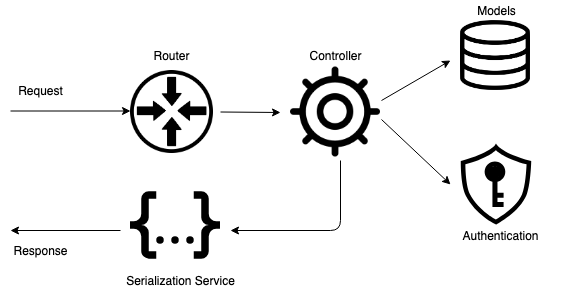
\includegraphics[scale=0.6]{figures/request_test.png}
            \caption{\label{request_test} Request Lifetime in Backend Service}
          \end{figure}

          Each route of the application is tested, exploring different possible
          scenarios for the incoming request (the idenfication token provided
          is invalid, the token is valid but the requested action is not
          authorized for the associated user). We therefore have a testing set
          that uses the whole application, simply by sending request and
          making expectations about the awaited response from the application.

      \subsection{Code Coverage - Simple Cov}

        We chose to use Simple Cov in combination of the testing applied to
        the Backend. This tool allow to measure the code coverage of Ruby
        application and to provide the developer with useful information
        thanks to its test execution analysis.\\

        Our ambition on the user part of the Splay project was a total recast of
        the services in more simple and maintainable ones, it was therefore
        obvious and simple for us to reach a total coverage of that new codebase
        with a test suite, and thus chose to use that tool.

      \subsection{Code Quality - Rubocop}

        we used Rubocop as the last piece of the tool stack designed to ensure
        the code quality within the service. Rubocop is a static code analysis
        tool (linter) allowing to detect violations to a set of rules about
        the code style and good practices (too many lines of code for a method,
        to many variables instanciations, too many conditional branching
        in the code, ...).

    \section{Testing in Daemons}


    \section{Integration Testing}

      In order to automatically test the project as a whole, we also wanted to
      develop a functional test suite. This test suite would be relatively
      simple but complete enough to make sure that we could test the developed
      features in a global way among the system, and to achieve this goal we
      just had to translate our user scenarios into test scenarios.\\

      For these functional tests, we didn't use a complex technology and
      thought that a Bash scripts serie would be more than sufficient to
      reach our goal. Bash scripts could indeed not allow us to recreate user
      behaviour using Splay through the web application, but as this
      application is using the exact same API offered by the Backend than the
      CLI application, we could simulate user behaviour through that CLI (and
      that's partially the reason why the decided to keep a CLI application
      within the project).\\

      The integration tests were placed in a dedicated directory at the Splay
      project's root, and execute the following actions for each test :

      \begin{itemize}
        \item Cleaning the containers.
        \item Rebuilding the different services listed in the docker-compose
        file.
        \item Starting up the services.
        \item Executing commands through the CLI.
        \item Checking the returned responsed sent by the CLI and displaying
        whether the test phase has succeeded or failed in the terminal.
      \end{itemize}

      {\color{red} Link with scenarios}\\

      By proceeding this way and with the fact of using our user scenarios to
      determine the actions described in the test suite, we can make sure
      that the implementation of our features is functional and will stay
      functional through the lifetime and evolutions of Splay. Moreover, those
      tests are adding an additional validation layer compared to the tests
      targeting the different services individually. We have here tests that
      are involving each service in concrete scenarios and reflecting real
      working conditions of the project, and also testing interactions
      between the services.

    \section{Continuous Integration}

      Once again in a way to ensure quality, the different services were placed
      on the Travis CI \cite{travis} continuous integration platform. Travis
      can be coupled with Github to detect any change on the branches and
      automatically run a test procedure listed in a script and then offer
      feedback on how the test suite went.\\

      Splay being an open source project, that we hope to see growing in the
      future, its collaborative development will inevitably happen through
      the Github organization in which the different repositories are located.\\
      The coupling of Travis with Github allow, in the case of a pull request,
      gather the review about the test execution on the branch asking to be
      merged with the main branch, and therefore to make sure the build is
      clean and the test are passing before merging the new code.

    \section{Overall Testing Suite}

      Here is a figure detailing the whole Splay project with the different
      test suites and procedures that have been described in the previous
      sections so that the reader can get the grasp on the overall
      organisation of this.

      \begin{figure}[H]
        \centering
        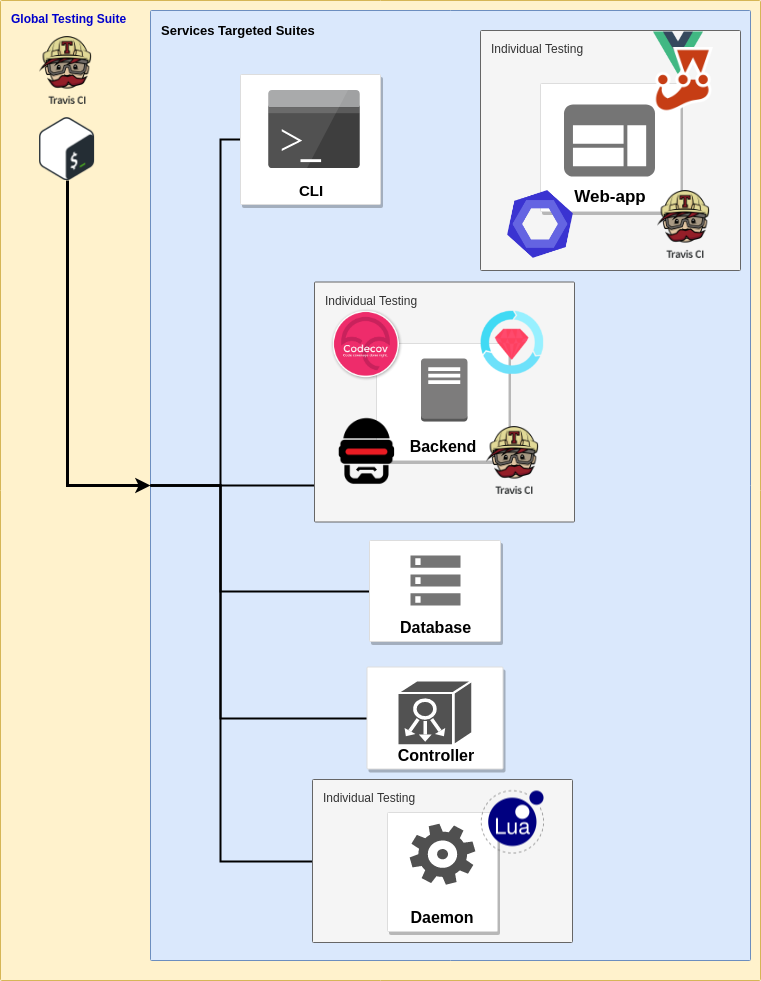
\includegraphics[scale=0.6]{figures/global_testing.png}
        \caption{\label{global_testing} Global Testing in Splay}
      \end{figure}

  \chapter{Use Case}
  A student wants to test his raft implementation
    \begin{itemize}
      \item The student register or connect to the Splay web server
      \item After doing the code of raft, he wants to try on several nodes (5),
      beginning without network topology (all nodes is directly connect).
      \item He sees the log to check if one node is leader and no more.
      \item He wants to test the correctness of his code by making crash the
      leader essentialy,
      but also the other.
      \item After checking his previous code, he repeats all process with and
      network topology.
    \end{itemize}


  \chapter{Conclusion}

    \section{Objective vs Done}

    \section{}

  \chapter{Improvements}


  \nocite{*}
  \bibliographystyle{plain}
  \bibliography{biblio.bib}




  % Back cover page
  \backcoverpage

\end{document}
